\subsection{MicroNet Tools}
\label{sub:tools}

The MicroNet tools are a collection of Eclipse plug-ins. Eclipse was chosen due
to the primary Java nature of MicroNet. This allows a quick development of Java
\mss{}. But the MicroNet tools also offer a way to integrate other
technologies into a \ms{} application. This language independence is
accomplished by using \gls{json} as a low level information exchange format. As
long as a technology supports \gls{json} it can participate in the application.
Another requirement is that it is possible to access to the message broker with
the foreign technology.

Since the \gls{ui} of an Eclipse plug-in is written using the Swing
Window Toolkit (SWT) library it can easily be exported to be a stand-alone tool
decoupled from Eclipse. With this approach it is possible to port the MicroNet
Tools to other platforms as long as they support a \gls{jvm}.

The MicroNet Tools have been completely developed within this last semester
thesis and are a major contribution to four of the hypotheses listed in
\autoref{sub:hypothesis}: the composition, deployment, simple development, and 
reproducibility hypotheses.

More information on the MicroNet Tools can be found in the MicroNet online
documentation \cite{micronet2017doku}.

\subsubsection{Files and Folders Structure}

To allow loose coupling of a \ms{} application MicroNet makes a few assumptions
on how to organize files and folders:

\begin{itemize}
  \item The eclipse workspace folder must contain one project folder for each
  \ms{}.
  \item For automated integration of a \ms{} its project folder must be either a
  Java/Maven project or it must contain a Dockerfile.
 \item One shared folder must be present to exchange the \textit{Shared Model} and the
  \textit{Service API}.
\end{itemize}  

\begin{figure}
	\centering
	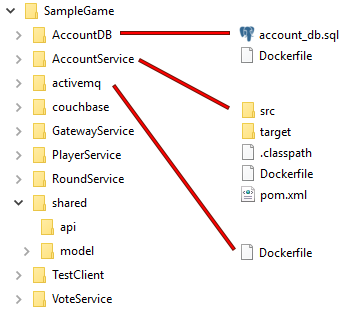
\includegraphics[width=9cm]{images/tools/folder_structure}
	\caption{Example folder structure of a MicroNet application workspace.}
	\label{fig:folder_structure}
\end{figure}

\autoref{fig:folder_structure} shows an example of a folder structure of a
MicroNet application workspace. The shared folder in this case is simply a folder within the
workspace. The figure also shows three canonical examples of project folders.
The AccountDB folder represents a containerized PostgreSQL database. The
AccountService folder is a standard MicroNet Maven/Java service project. The
activemq folder contains only a Dockerfile, which is the minimal requirement to
participate in a MicroNet application.

\subsubsection{Annotations}

MicroNet \textit{Annotations} provide a solution to define a \ms{} in a very
lean way. A service is defined by annotating an arbitrary class in the service
projects with the \textit{@MessageService(uri=``mn://service\_name'')}
\textit{Annotation}. Within the service class listener methods can be annotated
with the \textit{@MessageListener(uri=``/api\_method'')} \textit{Annotation} to
define the reactive behaviour of the service according to the defined \gls{api}.
Examples of services defined by the \textit{Annotation} can be seen in
\autoref{lst:service_communication} and \autoref{lst:message_parameters}.

\begin{figure}
\begin{lstlisting}[language=Java,firstnumber=1] 
@MessageService(uri = "mn://foo")
public class ServiceFoo {
	@OnStart
	public void onStart(Context context) {
		System.out.println("Start called");
	}
	
	@OnStop
	public void onStop(Context context) {
		System.out.println("Stop called");
	}
	
	@MessageListener(uri="/hello")
	@RequestPayload(UserValues.class) 
	@ResponsePayload(CredentialValues.class)
	@RequestParameters({
		@MessageParameter(code=ParameterCode.ID, type=Integer.class),
		@MessageParameter(code=ParameterCode.NAME, type=String.class)
	})
	@ResponseParameters({
		@MessageParameter(code=ParameterCode.ID, type=Integer.class),
	})
	public Response helloHandler(Context context, Request request) {
		int idParameter = request.getParameters().getInt(ParameterCode.ID);
		String nameParameter = request.getParameters()
			.getString(ParameterCode.NAME);
		
		UserValues user = Serialization.deserialize(
			request.getData(), UserValues.class);
		System.out.println("Process: " + user + " and " + nameParameter);

		String responseData = Serialization.serialize(user.getCredentials());
		Response response = new Response(StatusCode.OK, responseData);
		response.getParameters().set(ParameterCode.ID, idParameter);
		return response;
	}
}
\end{lstlisting}
\caption{A fully defined MicroNet \ms{} including all possible pre- and
post-condition \textit{Annotations}.}
\label{lst:pre_post_conditions}
\end{figure}

MicroNet \textit{Annotations} also provide a basic implementation of the design
by contract pattern. A service defines preconditions on request payloads and
defines post-conditions on response payloads. This system aims to prevent
semantic errors in communications. The pre- and post-conditions build the
foundation of the \textit{Code Assist} tool of MicroNet which helps the
developer in preventing mistakes in \ms{} communication design.
\autoref{lst:pre_post_conditions} shows a \ms{} defined by \textit{Annotations}
containing a well defined message listener with all pre- and post-conditions.
Theoretically the \textit{@RequestParameter} and \textit{@ResponseParameter}
\textit{Annotations} could implicitly be generated by parsing the \gls{ast} of
the listener method. This is however a very advanced topic which could fill a
whole thesis in itself.
 
 \paragraph{Annotation Processing}
 
Java annotations can either be used during run-time or processed during
compilation-time. MicroNet only processes \textit{Annotations} at compile-time.
Since Java version 6 the annotation processing process is tightly integrated
into the standard Java build process. This renders the \textit{Annotation}
process platform independent and it can be reproduced in a command line java
build, a Maven build or an Eclipse build\footnote{Annotation processing is
executed by the Java compiler which behaves slightly different for all evaluated
build setups (Eclipse, Maven, or Java native). Specifically newly generated
annotations are only found by the Eclipse proprietary compiler.}.

\textit{Annotation Processing} is also the entry point for code generation.
Even if no annotations are present in a project \textit{Annotation Processing}
can still be activated just to generate the \textit{Shared Model} and without
generating any service implementation. The MicroNet \textit{Annotation
Processor} provides an option for this purpose.

\subsubsection{Code Generation}

Code generation allows the developer to omit the boiler plate code that is
needed to integrate a service into a MicroNet application. This covers the setup
of the appropriate networking solution according to the environment and the
generation of the executable class of the \ms{}. This simplification allows the
developer to focus more on the actual domain logic of the \ms{}. It also spares
the developer having to register the main service class within the
application. The service class is automatically found and registration is
implicitly done by the \textit{Annotation Processor}.

The code generation library of MicroNet is very small and can be translated to
other programming languages very easily if needed. Since code generation is
basically nothing more than generating the right ``text-files'' this can be
accomplished in almost any imaginable programming language.

The MicroNet code generation library is implemented using the Java Poet
library. Java Poet allows for typesafe generation of Java classes and is very
easy to use. 

\paragraph{Service Generation}

The \textit{@MessageService} and \textit{@MessageListener} \textit{Annotations}
are used to build the executable class of a \ms{}. The executable class
registers all message listeners within the networking system. In addition the
annotated \textit{@Start} and \textit{@Stop} methods are called at service start
or at service termination respectively. The generated main method encompasses
the start/stop functionality and the listener registration in a defined set-up
sequence. \autoref{lst:generated_service} shows the generated implementation of
the annotated service shown in \autoref{lst:pre_post_conditions}.

\begin{figure}
\begin{lstlisting}[language=Java,firstnumber=1] 
public final class ServiceImpl {
  public static void main(String[] args) {
    try {
      System.out.println("Starting ServiceFoo...");

      IPeer peer = PeerFactory.createPeer();
      Context context = new Context(peer, "mn://foo");
      ServiceFoo service = new ServiceFoo();

      System.out.println("Registering message listeners...");
      peer.listen("/hello", (Request request) -> 
      	service.helloHandler(context, request));

      System.out.println("ServiceFoo started...");
      service.onStart(context);

      Runtime.getRuntime().addShutdownHook(new Thread() {
        @Override
        public void run() {
          System.out.println("ServiceFoo stopped...");
          service.onStop(context);
        }
      });
    }
    catch (Exception e) {
      System.err.println("Could not start ServiceFoo...");
      e.printStackTrace();
    }
  }
}
\end{lstlisting}
\caption{An executable \ms{} main class generated out of an annotated service
class.}
\label{lst:generated_service}
\end{figure}

\paragraph{Model Generation}

The model generation process is completely independent from the service
generation and is used to translate the game model which is defined in
\gls{json} to java POJOs (plain old Java objects). Because the MicroNet Model
generation library is very small it can also be reproduced in other programming
languages with relative ease. \autoref{lst:generated_model_class} shows the
\textit{UserValues} POJO generated out of the corresponding \textit{Template Type}
shown in \autoref{lst:template_type}.

\begin{figure}
\begin{lstlisting}[language=Java,firstnumber=1] 
public class UserValues {
  private int id;
  private CredentialValues credentials;

  public void setId(int id) {
    this.id=id;
  }

  public int getId() {
    return id;
  }

  public void setCredentials(CredentialValues credentials) {
    this.credentials=credentials;
  }

  public CredentialValues getCredentials() {
    return credentials;
  }
}
\end{lstlisting}
\caption{The UserValues POJO created out of the corresponding \textit{Template Type}.}
\label{lst:generated_model_class}
\end{figure}

The challenge for model generation is not the generation process itself but the
definition and editing process of the model that is generated and its
representation. These aspects make up a much larger part of MicroNet than the
actual code generation. Model editing and representation is further discussed
below in the paragraph on the \textit{Model Editor}.

\subsubsection{Code Assist}

The \textit{Code Assist} plug-in helps the developer to keep track of
functionality provided by other services. It presents the \textit{Service API}
in a type-safe way to the developer by relying on the pre- and postconditions
defined by MicroNet \textit{Annotations}.

\textit{Code Assist} is implemented by using the Eclipse code-completion
extension point. This extension point is used to add custom entries to the code
completion list box. This functionality is used to offer the MicroNet \gls{api}
to the developer any time he types \textit{``mn://''} in a source file. The
proposals are filtered according to the developer's input.

Type-safety enforcement is currently not implemented in MicroNet due to the same
reason as mentioned above in the section on \textit{Annotations} that require
parsing the \ms{} code. It could however be implemented by searching the
\gls{ast} of a message handler method for references on the request and response
objects. Calls to \code{getParameters()} or \code{setParameters()} can be
analyzed in regard to which \code{ParameterCode}s are used and which the
\textit{Template Type} of the parameter is. This feature would allow the
developer to omit the \code{@RequestParameters} and \code{@ResponseParameters}
\textit{Annotations}.

Upon violation of the message types the compiler can generate an error which
forces the developer to fix the issue before a build can be executed.
Although this process is possible the implementation of violation detection
again involves parsing the Java \gls{ast} and this effort is out of the scope of
this thesis.

In the current version of MicroNet the types are presented to the developer via
a tool-tip. Although type-safety is not enforced the developer can at least read
the correct types in the \textit{Code Assist} tool-tip, which alone is already
very helpful. \autoref{fig:code_assist} shows the \textit{Code Assist} tool-tip
for the \code{mn://foo/hello} message listener that was shown in 
\autoref{lst:pre_post_conditions}.

\begin{figure}
	\centering
	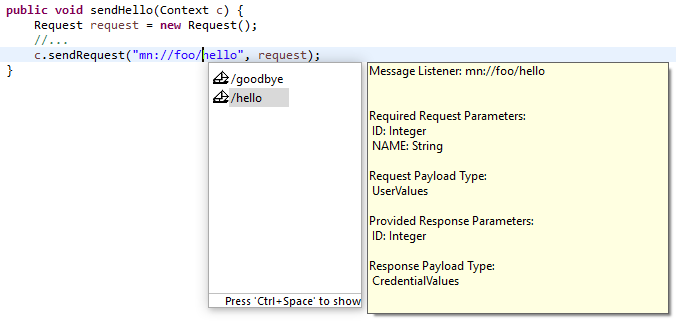
\includegraphics[width=\textwidth]{images/tools/CodeAssist}
	\caption{MicroNet \textit{Code Assist} tool-tip.}
	\label{fig:code_assist}
\end{figure}

\subsubsection{Service Explorer}

The \textit{Service Explorer} is the central management UI of a MicroNet and
helps the developer to get an overview over the whole game application. The
\textit{Service Explorer} is realized using a custom Eclipse view. The view
contains a list of all services showing their versions along with other useful
information like required ports or links to other services. The \textit{Service
Explorer} displays services which are Java, Maven and Docker projects. The
service list is dynamic and automatically refreshed when projects are created or
deleted.

The service list can be used to quickly edit the configuration of services. This
includes the port configuration as well as service linkage for the Docker
overlay network.

The \textit{Service Explorer} is also used to configure the composition of the
application in a visual way. Services can be activated to be part of the build
process, which automatically integrates them into the composition files (Maven:
pom.xml, Docker: docker-compose). This is done by deciding for each service
individually if it is part of the Maven build and/or part of the Docker
container build process.

The \textit{Service Explorer} also provides a quick interface to all launch
configurations explained in the \textit{Launch Utility} section below. The launch
functionality is provided with a context menu for each service in the list and
through the local pull-down menu offered by the Eclipse view.
\autoref{fig:service_explorer} shows the \textit{Service Explorer} with the
launch menu of the \code{FooService} open.

\begin{figure}
	\centering
	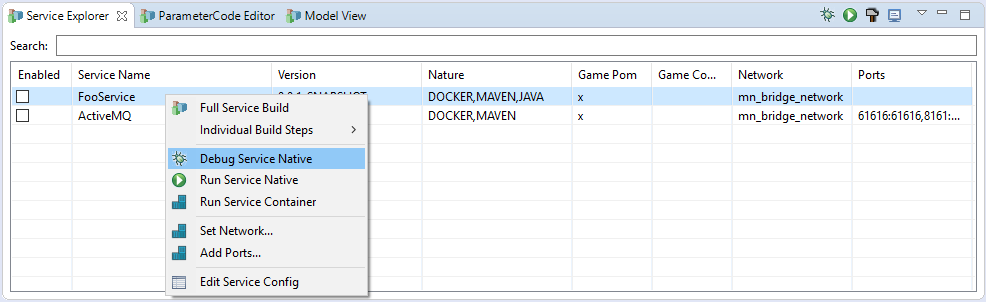
\includegraphics[width=\textwidth]{images/tools/ServiceExplorer}
	\caption{MicroNet \textit{Service Explorer}}
	\label{fig:service_explorer}
\end{figure}

\subsubsection{Launch Utility}

The \textit{Launch Utility} brings order to the vast different possibilities of
how to orchestrate a \ms{} application with containers. Many different configurations
can be helpful to develop, test and deploy a \ms{} application. The MicroNet
launch tools provide an easy way to set-up and start launch configurations.

The launch configurations of a Java/Maven build are offered via the Eclipse
Launcher plug-in. For these configurations the MicroNet \textit{Launch Utility}
only has to run the respective Eclipse Launch configuration.

Automation of the Docker container build process is not as simple because
Eclipse does not offer built-in functionality to access the Docker daemon.
The Docker Tools for Eclipse can be used to fulfill this gap since it provides
the necessary Docker container launch configurations. This however introduces a
strong dependency on the Docker Tools, which is undesirable. Many client for the
Docker daemon exist to integrate Docker automation into applications. This
however introduces another dependency closely related to Eclipse; and also the
tested Spotify Docker client which looks very promising has caused several class
path run-time errors and does not support Docker compose.

A workaround is to automate the Docker CLI using the Java run-time environment.
With this approach the docker commands are simply executed on the host of the
\gls{jvm}. This decouples the Docker integration mainly from Eclipse and places
it into the used Docker CLI. A Docker CLI is available for all major platforms:
Linux, Windows and MacOS. Since the docker CLI commands are the same on all
systems this is a platform independent approach since it only relies on a
\gls{jvm} and the docker CLI which is installed alongside Docker anyway. A
Drawback is that the developer has to configure the host-path to the docker CLI
executables. This is further complicated when Docker Toolbox instead of native
Docker is used since Docker Toolbox requires setting several Docker environment
variables. The MicroNet \textit{Launch Utility} however encompasses all this
functionality.

The \textit{Launch Utility} can deploy MicroNet applications in three distinct ways which
can all be combined which each other: local native, local containerized, and
cloud containerized. \autoref{fig:launch_utility} shows how the launch
configurations can be started via the \textit{Service Explorer}. The rest of this
paragraph explains all three deployment modes.

\begin{figure}
	\centering
	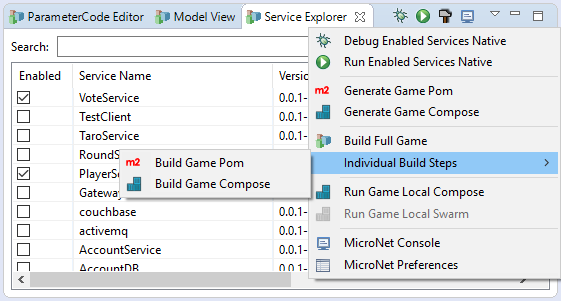
\includegraphics[width=14cm]{images/tools/LaunchUtility}
	\caption{\textit{Launch Utilities} offered by the \textit{Service Explorer}}
	\label{fig:launch_utility}
\end{figure}

\paragraph{Local Native}

\begin{figure}
	\centering
	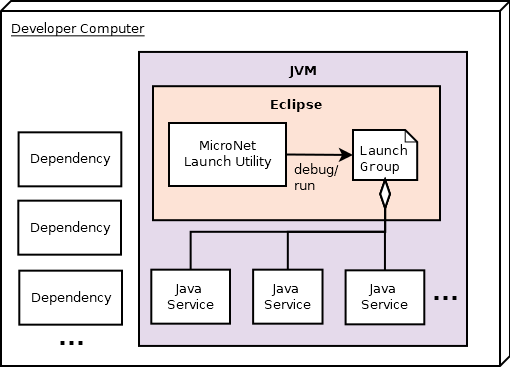
\includegraphics[width=10cm]{images/architecture/DeploymentLocalNative}
	\caption{Local native deployment of a MicroNet driven application.}
	\label{fig:deployment_local_native}
\end{figure}

The native configuration runs or debugs a game application as a set of native
Java applications. This makes debugging very fast and the integration in Eclipse
provides many useful debugging tools. To launch multiple Java applications at
once the CDT Launch Group plug-in is used. It composes multiple launch
configurations into a single configuration. Upon Launch Group execution all
contained applications are individually started. No build step is further needed
for this configuration.

For native configurations it is easiest to run software on which the application
depends as stand-alone installations on the host. Since the native configuration
is solely used during development this also allows the dependencies to be tested
isolated from the composed application. It is nonetheless possible to combine a
local native configuration with a local containerized configuration. Services
and dependencies can therefore be started in the configuration best suited for
them.

\autoref{fig:deployment_local_native} shows the deployment of a MicroNet
driven game in local deployment mode.

\paragraph{Local Containerized}

The local containerized configuration is meant to reproduce the final deployment
process on the local developer machine. For this purpose Maven and Docker
compose/swarm are used. 

A local Maven build of the complete application is done by aggregating the
individual Maven service projects into a master .pom file. The master .pom can
be used to build the whole application at once. The kind of services that are
aggregated to the master .pom file can be configured via. the \textit{Service Explorer}.

A local Docker deployment is defined by a docker-compose file. This file is also
defined by configuring services via the \textit{Service Explorer}. The Docker build
process is then simply invoked by building the docker-compose file.

In order to run the local containerized application the local docker engine can
be used. Docker-compose is natively installed with most docker installations or
can be separately installed. The application can be started locally either using
Docker-compose or docker swarm commands. On the local developer machine there is
only little difference between docker-compose and -swarm. Networking however
behaves differently locally and in the cloud so the local networking
configuration cannot be identically transferred to the cloud environment.

\begin{figure}
	\centering
	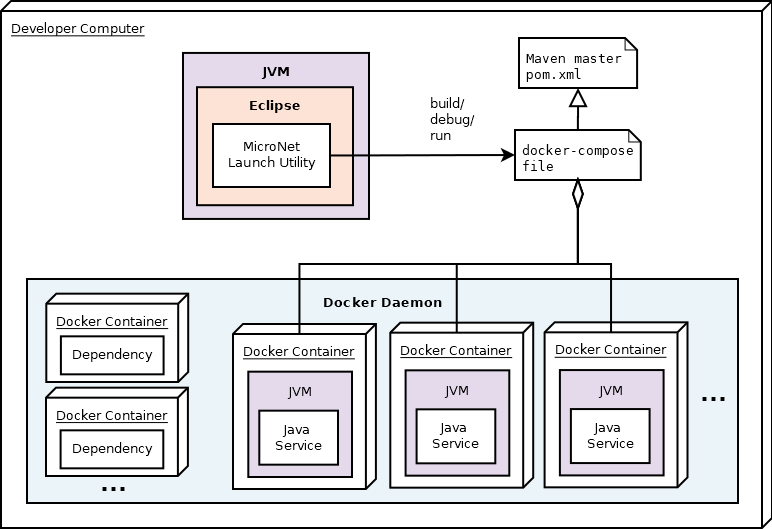
\includegraphics[width=\textwidth]{images/architecture/DeploymentLocalContainerized}
	\caption{Local containerized deployment of a MicroNet driven application.}
	\label{fig:deployment_local_containerized}
\end{figure}

\autoref{fig:deployment_local_containerized} shows how an application is
composed and deployed in the local containerized mode.

\paragraph{Cloud Containerized}

The final step of \ms{} application deployment is cloud deployment. The idea
behind application containerization is that this process is meant to be
deterministically reproducible on different systems. Therefore if the
application is working in the local containerized configuration the cloud
configuration can be achieved in a similar way.

MicroNet does not provide any out-of-the box solution to automatically deploy an
application in the cloud. This is because of the variety of
different infrastructures that can be used to deploy MicroNet. But the
deployment is prepared by MicroNet so it can be done with very few console
commands via SSH.

Due to the restrictions mentioned in \autoref{sub:zero_buget} the production
environment of \mn{} is a virtual Linux server in the HSR cloud. The cloud
deployment process is mainly based on this environment. Since this a very
general setup the process can easily be reproduced on other environments.

In order to deploy a MicroNet \ms{} application the developer must perform the
following steps under the assumption that the server runs a fresh Linux
installation.

\begin{itemize}
  \item Install: Docker Engine, Java, Maven and Git.
  \item Initialize docker swarm (master and worker machines).
  \item Pull the game application repository via Git (containing all service
  projects and the shared folder).
  \item Build the application class files using the master .pom file (annotation
  processing and code generation is performed during this step).
  \item Containerize the application using docker-compose \gls{api} and the generated
  docker-compose file.
  \item Launch the application in Docker Swarm using the docker stack \gls{api}.
\end{itemize}

\begin{figure}
	\hspace*{-0.8cm}
	\centering
	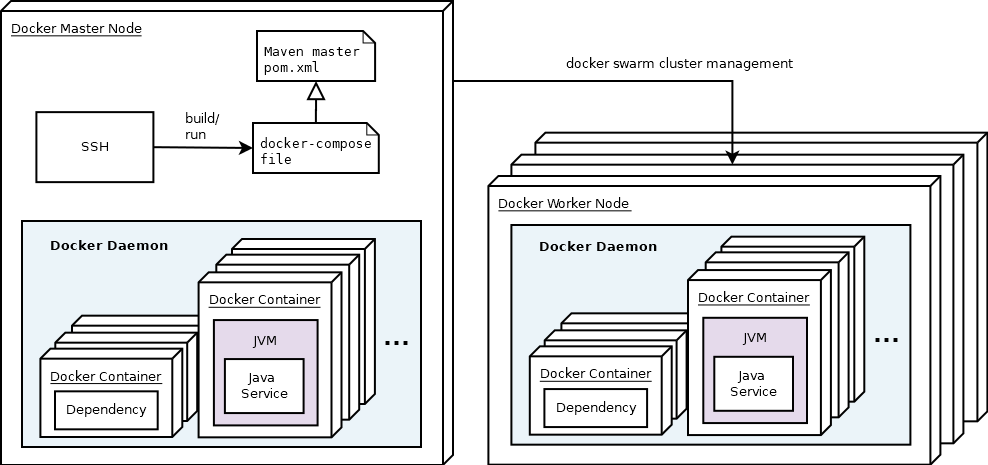
\includegraphics[width=1.1\textwidth]{images/architecture/DeploymentCloudContainerized}
	\caption{Cloud containerized deployment of a MicroNet driven application.}
	\label{fig:deployment_cloud_containerized}
\end{figure}

This sounds like a lot of steps but in fact the process is reasonably quick and
only requires very few console commands which can be looked up in the MicroNet
documentation \cite{micronet2017doku}.
\autoref{fig:deployment_cloud_containerized} gives an impression on how such a
docker-swarm environment may look like.

\subsubsection{Model Editor}

The \textit{Model Editor} is the last feature that was introduced in MicroNet
tools. It is the final solution for how to cope with logical \ms{} composition
through the \textit{Shared Model} in a visual way. Since the game model is
designed to be mainly machine-readable it is not suited to be directly edited in
the underlying \gls{json} files. The \textit{Model Editor} is designed to allow
convenient defining and editing of the model in a way which is especially useful
for \og{} application.

The \textit{Model Editor} is basically a graph editor visualizing a direct
representation of the game graph to allow extending and changing the graph. The
graph has three root nodes each of which span a model tree: the parameter code
list, the \textit{Template Tree}, and the \textit{Prefab Tree}.

\paragraph{Parameter Code List}

The parameter code tree is simply a flat list of String constants which define
all the parameter codes used throughout the application. This global approach
allows the substitution of the parameter codes strings with numbers, which is
more space efficient. Since parameters are used very often this has a noticeable
impact on the bandwidth requirements of an application.

\paragraph{Template Tree}

The \textit{Template Tree} allows to edit the game's \textit{Template Types}
using graph editing. Object Types defined using the \textit{Template Tree} can
be used for message transfer and persistence. \textit{Template Type} are
descriptions of domain objects and are used to generate \textit{Shared Model}
classes (POJOs) during code generation.

A \textit{Template Type} consists of a set of fields that may be of the
following types: STRING, NUMBER, BOOLEAN, CHAR, ENUM, LIST, SET, MAP, and
COMPONENT. The types are derived from the Java types since they are well
documented and can be redefined in other programming languages using the Java
language specifications.

The COMPONENT type can be any other \textit{Template Type}. A component is
represented as a field in the data class. Also \textit{Template Types} can be
derived from other \textit{Template Types}. The derivation is realized using
regular Java inheritance. \autoref{fig:model_view} shows the \textit{Model
Editor} which can be used to manually edit the \textit{Template Tree}.

\begin{figure}
	\centering
	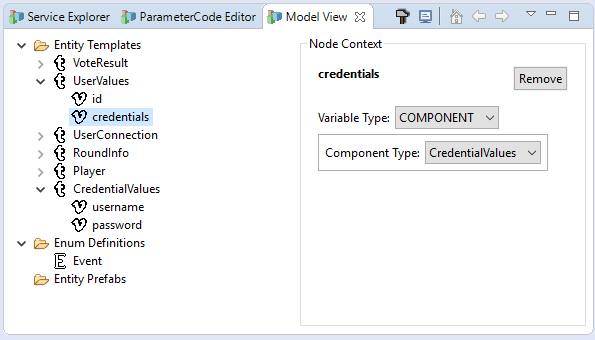
\includegraphics[width=\textwidth]{images/tools/ModelView}
	\caption{\textit{Template Type} editing with the MicroNet \textit{Model Editor}.}
	\label{fig:model_view}
\end{figure}

\paragraph{Prefab Tree}

The \textit{Prefab Tree} is a ``physical'' instantiation of the game graph. It
contains actual instances of \textit{Template Types}. This can be used by game
designers to pre-define game objects that are later used in the game. The
\textit{Prefab Tree} is directly compatible with the serialization component
provided by MicroNet. The generated model classes which represent the
\textit{Template Types} can be used to directly serialize and de-serialize game
objects which are part of the prefab-tree. The serialized data can directly be
stored in the database or be used as a payload or as parameters for message
transfers.

The \textit{Prefab Tree} can either be persisted in the file-system or persisted in the
database in \gls{json} format. The \textit{Prefab} approach allows for very
convenient and consistent handling of game data both during development and
operation.

